\newpage
\begin{center}
    \section{Mon rôle en tant que stagiaire: fraisage, découpe, lecture de plan}
\end{center}

\subsection{AMOI: Atelier Métallique Océan Indien}
% 1, 2, 3, 6 et 7 (ne pas hésité à mettre des sous section)

\subsubsection{Place et fonction du service}% 1 et 2
L'atelier AMOI, à pour objectif la réalisation des structures (charpente métallique, gros œuvres, installation sur chantier...) dont les plans sont fournis par les dessinateur de SMOI. Ce service à donc pour fonction la réalisation physique des demandes des clients.

\subsubsection{Moyen matériel et humain du service}% 3 et 6
L'atelier est composé de six salariés, trois ouvriers de chantier, un responsable de l'atelier, un chargé de la quincaillerie et un chargé de la peinture et des revêtements. Il est alors séparer en cinq parties:
\begin{enumerate}
    \item L'entrepôt des matières première et/ou des produit en cours de transformation
    \item L'entrepôt des outils, corde, échelle, la quincaillerie
    \item Un espace dédié à la pose de peinture et de revêtement
    \item Un espace dédié aux machine, pour la découpe, la soudure, le pliage, la transformation des matière première
    \item Un espace dédié au vestiaire
\end{enumerate}
Les principaux matériaux transformés dans l'atelier sont le fer, l'aluminium, l'inox et la tôle. Il sont alors transformés à l'aide de différente machine tel que une machine à découpe plasma\footnote{cf lexique p14}, une plieuse \ref{fig:plasma_plie}, une fraiseuse\footnote{cf lexique p14}, une machine de scie à eau, une presse hydraulique mais également des outils tel que des perceuses magnétique, des foreuse portable et des ponceuse.
\begin{figure}[h!]
    \centering
    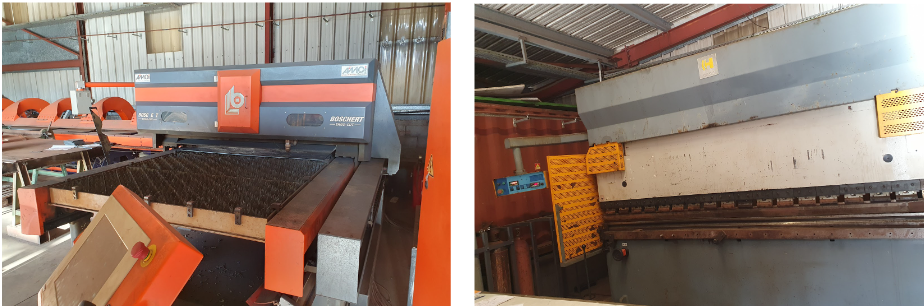
\includegraphics[width=1\linewidth]{figures/plasma_plie.png}
    \caption{Machine à découpe plasma \& Machine plieuse de tôles}
    \label{fig:plasma_plie}
\end{figure} \newpage
Étant donnée de cette équipe réduite, les communications en interne sont simplifiées. En effet, les interactions entre les autres services et l'atelier passe principalement par le responsable de l'atelier qui reçoit les dessinateurs pour faire le point sur les commandes avenir et les délais. De plus, comme l'équipe est réduite, l'organisation de réunion entre elle est peu compliquée et contraignante.\newline
En externe j'ai pu constater qu'il y avait des réunions avec les clients et que les fournitures passait principalement par commande téléphonique.\par

\subsubsection{Des dysfonctionnement matériel inquiétant}% 7
Cependant lors de mon stage l'entreprise a dû faire face à la panne de leur machine plieuse de tôles ralentissant alors fortement leur activité dans ce secteur durant presque plus d'un mois. Il y a tous au long de mon stage dans cette entreprise, eu la visite de réparation dans le but de réaliser les mise à jour nécessaire sur la machine et la remettre en état, cependant cela c'est avéré vain. Il a donc été pris la décision de remplacer la machine. Une opération délicate puisque nécessitant la venue d'une grue et le démantèlement d'une partie du toit de l'atelier.


\subsection{Mon activité de stagiaire}
% 4, 5 et 8 (une sous section pour chaque activité réalisé + une sous section général pour les info général)

Lors de mon stage j'ai travaillé de 8h à 12h puis de 13h à 16h du lundi au jeudi et de 8h à 12h le vendredi. Mes tâches étaient réparties en fonction de ce qui était disponible et des missions sur lesquelles l'atelier travaillait. Mais j'ai principalement réalisé des tâches de fraisages et lecture de plan de début de semaine et des tâches de nettoyage en fin de semaine.
\subsubsection{Fraisage}
La première et principale tâche que j'ai réalisée lors de mon stage était du fraisage, mais pour celle-ci on m'a expliqué le fonctionnement des machines (donc ici de la fraiseuse et des perceuses magnétiques). Je devais donc en suivant les cotations et norme imposée sur les plan et dessiner sur les barre de métal découper, percer des trou avec les bonne fraise, soit en utilisant une perceuse magnétique pour les barre de métals trop grosse et grande pour la fraiseuse, soit en utilisant la fraiseuse afin de réaliser des trou qui avait pour certain but d'être boulonné mais pour d'autre but de servir d'emplacement pour des vis. J'ai notamment réaliser le perçage de plaque servant à la réalisation d'un escalier, il fallait donc que j'utilise la fraiseuse avec une fraise spécifique de tel manière à percer précisément une plaque (sans pour autant la perforé entièrement) pour permettre le passage de vis à bois.
\subsubsection{gravure}
Après avoir perforé correctement les pièces métalliques, je me suis servi d'une machine à gravure par percussion afin de noter les référence de chacune des pièces (référence noté sur les schémas de coupes) pour pouvoir les entreposer en attendant la prochaine étape de leur transformation.
\subsubsection{Lecture de plan}
Une autre de mes tâche était la lecture de cotation sur les différents plan de coupes, assemblages\footnote{cf annexe 5} et pliages et de noter, dessiner avec précision sur les pièce considérer le marquage nécessaire pour la réalisation de pliage (notamment pour les tôles), le fraisage et la découpe. Une étape nécessitant une grande précision et dont le travail réalisé est systématiquement contrôlé avant toute autres actions de pliage ou de découpe.
\subsubsection{Découpe}
J'ai opéré deux type de découpe durant mon stage:
\begin{itemize}
    \item Une découpe plasma: On ne m'a pas appris le fonctionnement précis et l'utilisation du logiciel permettant le pilote de la machine, mais j'étais chargé de surveiller le fonctionnement de la machine qui avait quelques bugs et pour qui le programme devait être redémarer si cela arrivait. Je devais, à la suite du découpage, démouler les pièces des plaques découpées, les annoter de leurs références, les nettoyer en utilisant soit un burin, soit en utilisant une ponceuse puis percer les trous mal formés lors de la découpe et de les graver après soudure.
    \item Une découpe à l'eau: J'ai également reçu pour mission de réaliser des découpes précises de barres de métaux et/ou d'aluminium en utilisant une scie à eau. Je devais donc aller chercher les matières premières entreposées, les placer sur la machine en suivant les cotation du schéma de coupe et vérifier en fin de coupe la longueur si la longueur coupé était bien celle attendue.
\end{itemize}
\subsubsection{ponçage/meulage}
J'ai aussi réalisé du ponçage et du meulage, qui était pour mes mission, des mission de nettoyage des pièce intermédiaire, tel qu'avec une ponceuse, j'ai enlever les traces de la présence de point de soudure.
\subsubsection{pliage}
Une fois le remplacement de la machine de pliage effectué, j'ai pu non pas réalisé du pliage seul mais aider au maintien et placement des tôles pour leur pliage.
\subsubsection{montage}
Je suis également partie sur un chantier\footnote{cf annexe 6}, ici chez un particulier (un cabinet médical), dans lequel j'ai participé à l'installation d'une passerelle préalablement fabriquée dans l'atelier. J'ai donc participé à l'installation des piliers de celle-ci en forant les trous dans le sol pour y installer les vis allant dans les pieds des piliers. Je n'ai cependant, puisque n'ayant pas les habilitations nécessaires pour les travaux en hauteur, pas pu énormément participé quant à l'installation de la partie haute de la passerelle.\ref{fig:pillier_passerelle}
\begin{figure}[h!]
    \centering
    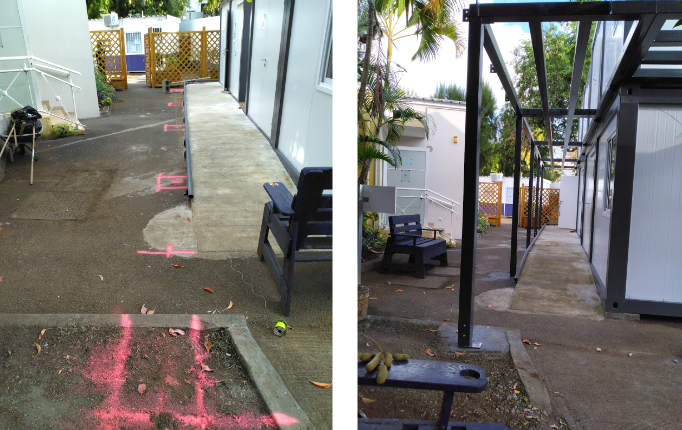
\includegraphics[width=1\linewidth]{figures/pillier_passerelle.png}
    \caption{photo de la passerelle avant et après installation des piliers}
    \label{fig:pillier_passerelle}
\end{figure}
\subsubsection{nettoyage}
La dernière tâche que j'ai réalisé à été de nettoyer, en passant le balais dans l'atelier, en triant les matières premières usées mais également en nettoyant les machine, notamment, la machine à découpe plasma avec l'aide du responsable de l'atelier.


\subsubsection{Conclusion}
%mini conclusion et résumé des info de la partie

Pour conclure cette partie, j'ai réalisé les principales tâche de la conception d'un produit à travers la fabrication des pièce intermédiaire pour l'assemblage, des activité qui chez moi ont suscité de l'intérêt avec des questionnement et recherche d'explication sur leur fonctionnement (des machine mais aussi des méthode de fabrication). Et cela malgré les péripéties survenu durant mon stage avec la panne d'une machine.
